\documentclass[12pt,a4paper]{article}

% Encoding & language
\usepackage[utf8]{inputenc}
\usepackage[T1]{fontenc}
\usepackage{amsmath,amssymb,amsthm}
\usepackage{booktabs,longtable,multirow}
\usepackage{graphicx}
\usepackage{geometry}
\usepackage{hyperref}
\usepackage{caption}
\usepackage{xcolor}
\usepackage{listings}
\usepackage{float}
\usepackage{siunitx}

\geometry{top=2.5cm,bottom=2.5cm,left=2.5cm,right=2.5cm}

\hypersetup{
    colorlinks=true,
    linkcolor=blue,
    citecolor=blue,
    urlcolor=blue
}

\lstset{
    basicstyle=\ttfamily\small,
    breaklines=true,
    frame=single,
    numbers=left,
    numberstyle=\tiny\color{gray},
    captionpos=b
}

\title{\textbf{ELEC9123 Design Task B}\\[0.3em]
\large Performance Analysis Verification via Monte Carlo Simulations}
\author{YU \quad zID: z5615351}
\date{\today}

\begin{document}

\maketitle

\begin{abstract}
This report presents a Monte Carlo simulation study for a BPSK system operating over six wireless channel models: AWGN, Laplacian impulsive noise, Rayleigh fading with AWGN, Rician fading with AWGN, and randomly deployed users over Rayleigh/Rician fading channels. The simulated bit error rate (BER) and outage probability are compared with their analytical counterparts. Results confirm close agreement between simulation and theory, with the residual deviations explained by the finite number of Monte Carlo samples.
\end{abstract}

\tableofcontents
\newpage

%=============================================================================
\section{Introduction}
%=============================================================================
The design task aims to verify key performance metrics of a BPSK wireless communication system through Monte Carlo simulations. Monte Carlo methods generate a large number of random channel and noise realisations, evaluate the system response for each realisation, and then assemble empirical probabilities that can be compared with theoretical expressions.

The report is organised as follows. Section~\ref{sec:parameters} lists the system parameters. Section~\ref{sec:laplace} describes the generation and verification of Laplacian noise. Sections~\ref{sec:ber} and~\ref{sec:outage} present the BER and outage probability methodologies, respectively. Section~\ref{sec:results} shows the numerical results and figures. Section~\ref{sec:discussion} discusses the observed deviations and the effect of sample size. Conclusions are drawn in Section~\ref{sec:conclusion}.

%=============================================================================
\section{System Parameters}\label{sec:parameters}
%=============================================================================
The default parameters used throughout the simulations are listed in Table~\ref{tab:parameters}.

\begin{table}[H]
\centering
\caption{System Parameters}
\label{tab:parameters}
\begin{tabular}{lll}
\toprule
\textbf{Parameter} & \textbf{Symbol} & \textbf{Value} \\
\midrule
Outage threshold & $C$ & \SI{1.2}{bps/Hz} \\
SNR range & $\gamma_b$ & $0$ to \SI{15}{dB}, step \SI{1}{dB} \\
Cell radius & $R$ & \SI{3}{m} \\
Path-loss exponent & $\nu$ & $2.2$ \\
LOS magnitude & $h_d$ & $1$ \\
Rician $K$-factor & $K$ & $5$ \\
Noise variance & $N_0$ & $1$ \\
Monte Carlo samples per SNR & $N$ & $10^6$ \\
\bottomrule
\end{tabular}
\end{table}

The outage SNR threshold is
\begin{equation}
    \gamma_{\text{th}} = 2^C - 1.
\end{equation}

%=============================================================================
\section{Laplacian Random Variable Verification}\label{sec:laplace}
%=============================================================================
Impulsive noise is modelled as a real Laplacian random variable with variance $N_0$. Using the scale parameter $b=\sqrt{N_0/2}$, the PDF and CDF are
\begin{align}
    f_n(x) &= \frac{1}{2b}\exp\!\left(-\frac{|x|}{b}\right), \\
    F_n(x) &=
    \begin{cases}
        \frac{1}{2}\exp\!\left(\frac{x}{b}\right), & x \le 0, \\[0.5em]
        1 - \frac{1}{2}\exp\!\left(-\frac{x}{b}\right), & x > 0.
    \end{cases}
\end{align}

Samples are generated via the inverse-CDF method:
\begin{equation}
    x = -b\,\text{sign}(u-0.5)\,\log\bigl(1 - 2|u-0.5|\bigr), \qquad u \sim \mathcal{U}(0,1).
\end{equation}

Figure~\ref{fig:laplace} compares the empirical PDF and CDF with the analytical expressions. The maximum absolute CDF error over the plotted range is approximately $9.3\times 10^{-4}$, confirming the correctness of the generator.

\begin{figure}[H]
    \centering
    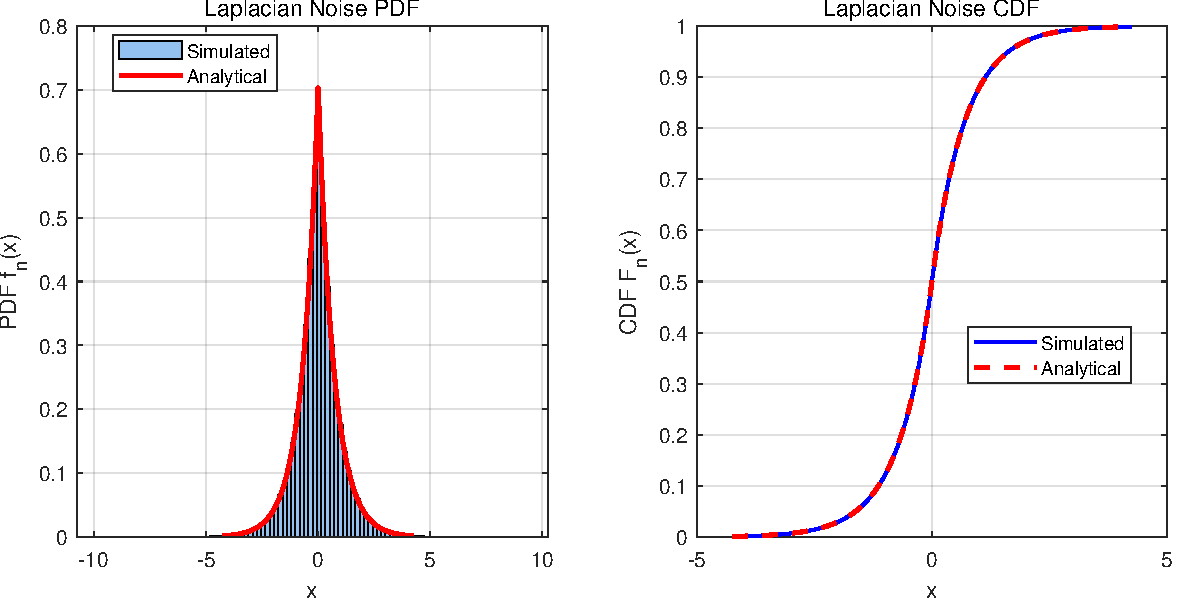
\includegraphics[width=0.95\textwidth]{figs/figure_1.pdf}
    \caption{Laplacian noise verification. Left: simulated histogram versus analytical PDF. Right: simulated empirical CDF versus analytical CDF.}
    \label{fig:laplace}
\end{figure}

%=============================================================================
\section{Bit Error Rate Simulation}\label{sec:ber}
%=============================================================================
For BPSK with coherent detection, the transmitted symbol is $x\in\{-1,+1\}$ with equal probability. The received signal in each channel is processed by the appropriate detector, and the empirical BER is the fraction of decoded bits that differ from the transmitted bits.

%-----------------------------------------------------------------------------
\subsection{Noise-only channels}
%-----------------------------------------------------------------------------
\paragraph{AWGN.} The received signal is $r = \sqrt{E_b}x + n$, where $n\sim\mathcal{CN}(0,N_0)$. The analytical BER is
\begin{equation}
    P_b^{\text{AWGN}} = \frac{1}{2}\operatorname{erfc}\!\left(\sqrt{\gamma_b}\right).
\end{equation}

\paragraph{Laplacian noise.} The received signal is $r = \sqrt{E_b}x + n$ with real Laplacian noise. The analytical BER is
\begin{equation}
    P_b^{\text{Lap}} = \frac{1}{2}\exp\!\left(-\sqrt{2\gamma_b}\right).
\end{equation}

%-----------------------------------------------------------------------------
\subsection{Flat-fading channels}
%-----------------------------------------------------------------------------
\paragraph{Rayleigh fading.} The fading coefficient $h_s$ is complex Gaussian with $E\{|h_s|^2\}=1$. After maximal-ratio combining (single-tap equalisation), the analytical BER is
\begin{equation}
    P_b^{\text{Ray}} = \frac{1}{2}\left(1 - \sqrt{\frac{\gamma_b}{1+\gamma_b}}\right).
\end{equation}

\paragraph{Rician fading.} The channel is $h = \sqrt{\frac{K}{K+1}}h_d + \sqrt{\frac{1}{K+1}}h_s$, with $E\{|h|^2\}=1$. The BER can be written via the MGF of the instantaneous SNR:
\begin{equation}
    P_b^{\text{Ric}} =
    \frac{1}{\pi}\int_{0}^{\pi/2}
    \frac{(K+1)\sin^2\theta}{(K+1)\sin^2\theta + \gamma_b}
    \exp\!\left(-\frac{K\gamma_b}{(K+1)\sin^2\theta + \gamma_b}\right)
    \,d\theta.
\end{equation}

%-----------------------------------------------------------------------------
\subsection{Randomly deployed users}
%-----------------------------------------------------------------------------
Users are uniformly distributed in a disk of radius $R$, so the distance PDF is $f_d(d)=2d/R^2$, $0\le d\le R$. Path loss is $d^{-\nu}$.

\paragraph{Rayleigh fading with random deployment.} Conditional on distance $d$, the average SNR is $\gamma_b/d^\nu$ and
\begin{equation}
    P_b^{\text{RayRand}}(d) =
    \frac{1}{2}\left(1 - \sqrt{\frac{\gamma_b}{d^\nu + \gamma_b}}\right).
\end{equation}
The unconditional BER is obtained by averaging over $f_d(d)$.

\paragraph{Rician fading with random deployment.} Conditional on $d$, the Rician $K$-factor is unchanged because both LOS and scattered components are attenuated by the same path-loss factor. The conditional BER is $P_b^{\text{RicRand}}(d)=P_b^{\text{Ric}}(\gamma_b/d^\nu,K)$, averaged over $f_d(d)$.

%=============================================================================
\section{Outage Probability}\label{sec:outage}
%=============================================================================
Outage occurs when the instantaneous capacity falls below $C$:
\begin{equation}
    P_{\text{out}} = \Pr\left\{\log_2(1+\gamma) < C\right\}
    = \Pr\left\{\gamma < \gamma_{\text{th}}\right\},
    \qquad \gamma_{\text{th}} = 2^C - 1.
\end{equation}

For the four outage scenarios:
\begin{align}
    P_{\text{out}}^{\text{Ray}} &= 1 - \exp\!\left(-\frac{\gamma_{\text{th}}}{\gamma_b}\right), \\
    P_{\text{out}}^{\text{Ric}} &= 1 - Q_1\!\left(\sqrt{2K},\sqrt{2(K+1)\frac{\gamma_{\text{th}}}{\gamma_b}}\right), \\
    P_{\text{out}}^{\text{RayRand}} &=
    1 - \frac{2}{\nu R^2}
    \left(\frac{\gamma_{\text{th}}}{\gamma_b}\right)^{-2/\nu}
    \gamma\!\left(\frac{2}{\nu}, \frac{\gamma_{\text{th}}R^\nu}{\gamma_b}\right), \\
    P_{\text{out}}^{\text{RicRand}} &=
    \frac{2}{R^2}\int_{0}^{R}
    d\left[1 - Q_1\!\left(\sqrt{2K},\sqrt{2(K+1)\frac{\gamma_{\text{th}}d^\nu}{\gamma_b}}\right)\right]
    \,dd,
\end{align}
where $\gamma(s,x)$ is the lower incomplete gamma function and $Q_1(\cdot,\cdot)$ is the Marcum $Q$-function.

%=============================================================================
\section{Results}\label{sec:results}
%=============================================================================
All simulations use $N=10^6$ samples per SNR point. Tables~\ref{tab:ber_dev} and~\ref{tab:outage_dev} list the percentage deviation between simulated and analytical results.

\input{tables}

Figures~\ref{fig:ber_noise}--\ref{fig:outage} present the BER and outage curves. The simulated curves follow the analytical curves closely across the SNR range.

\begin{figure}[H]
    \centering
    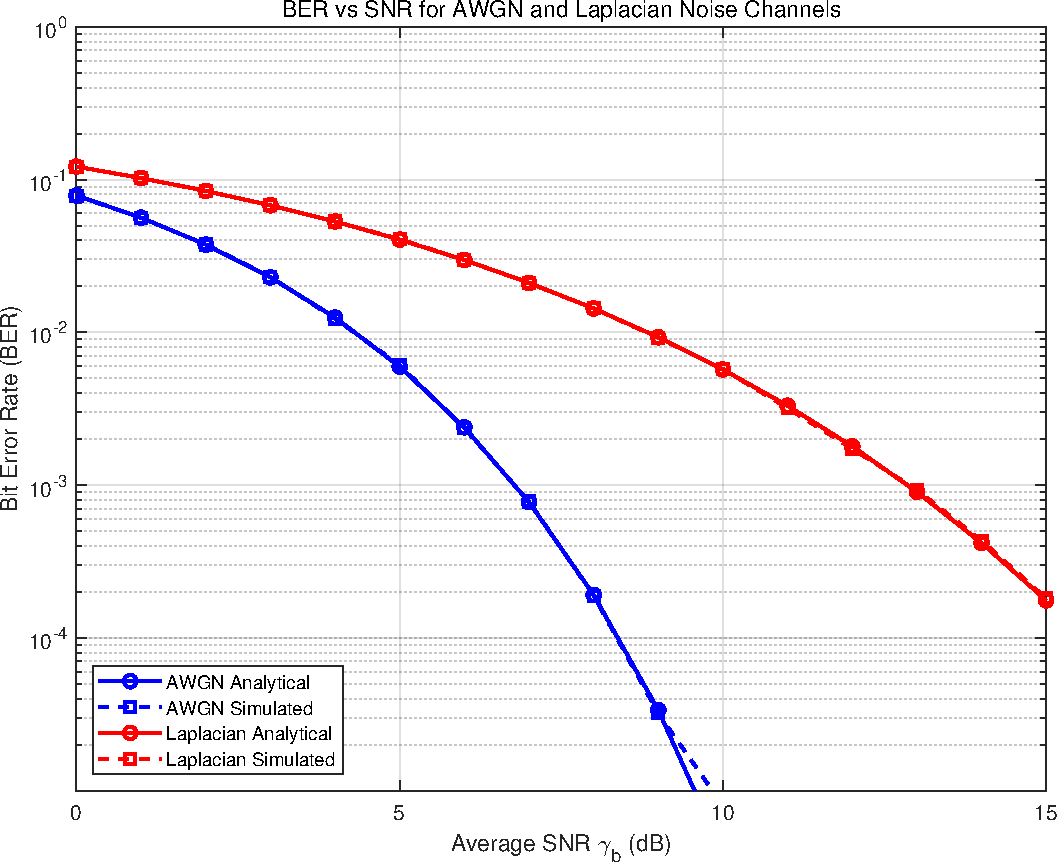
\includegraphics[width=0.85\textwidth]{figs/figure_2.pdf}
    \caption{BER versus average SNR for noise-only channels (AWGN and Laplacian impulsive noise).}
    \label{fig:ber_noise}
\end{figure}

\begin{figure}[H]
    \centering
    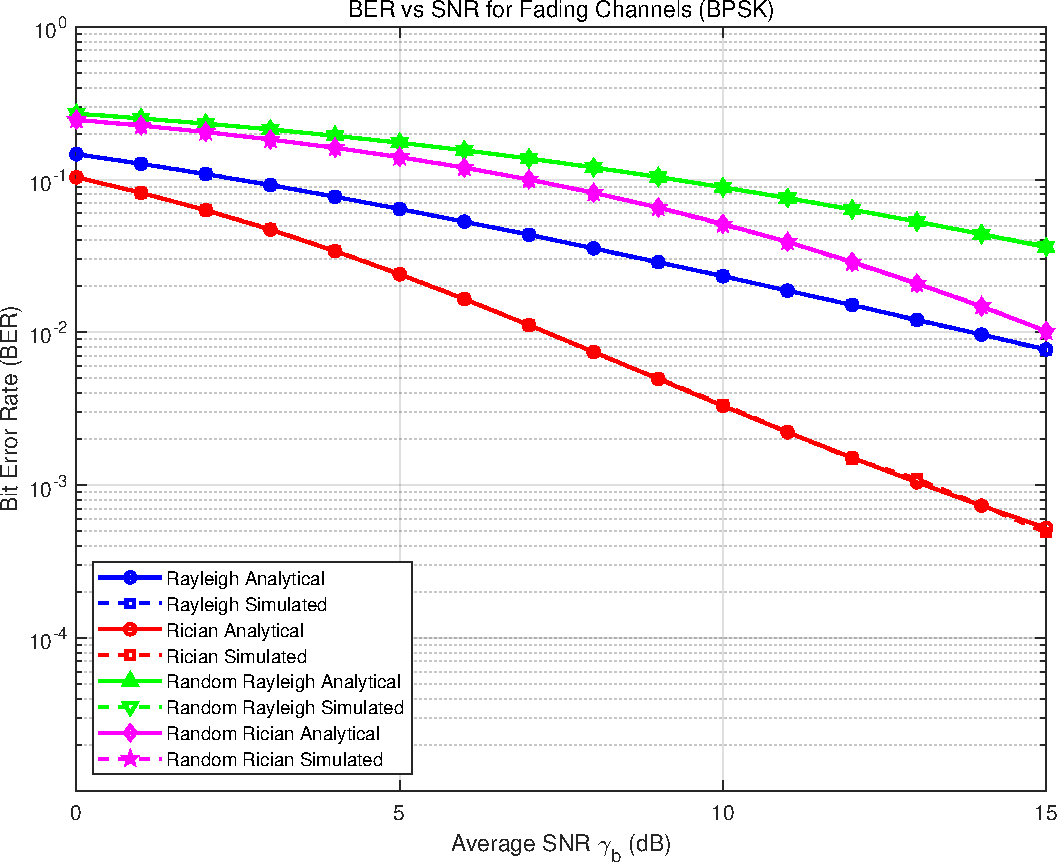
\includegraphics[width=0.85\textwidth]{figs/figure_3.pdf}
    \caption{BER versus average SNR for fading channels.}
    \label{fig:ber_fading}
\end{figure}

\begin{figure}[H]
    \centering
    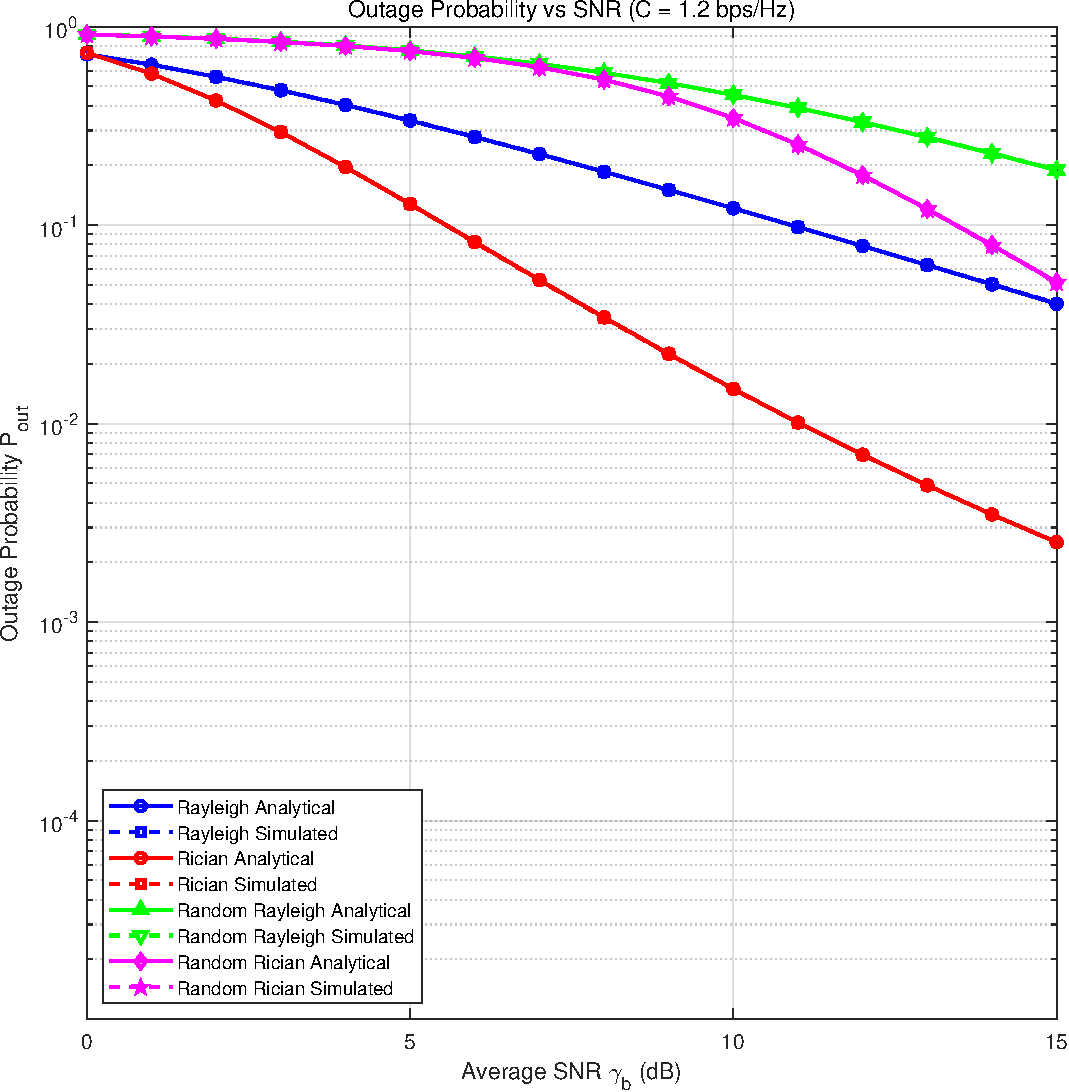
\includegraphics[width=0.85\textwidth]{figs/figure_4.pdf}
    \caption{Outage probability versus average SNR.}
    \label{fig:outage}
\end{figure}

%=============================================================================
\section{Discussion}\label{sec:discussion}
%=============================================================================
The outage probability deviations in Table~\ref{tab:outage_dev} are all below \SI{1}{\percent}, confirming the correctness of the outage simulation and analytical formulas.

For BER, the fading-channel deviations are generally within a few percent. The largest deviations occur for the AWGN channel at high SNR (10--\SI{15}{dB}), where the theoretical BER falls below $10^{-6}$. With only $10^6$ samples, zero or very few bit errors are observed, so the empirical BER is dominated by statistical fluctuations. This is a Monte Carlo sample-size limitation rather than an implementation error.

Table~\ref{tab:sample_conv} illustrates the effect of increasing $N$ for the AWGN channel at \SI{10}{dB}. As $N$ grows, the simulated BER approaches the analytical value, demonstrating that the Monte Carlo estimate converges with sample size.

%=============================================================================
\section{Conclusion}\label{sec:conclusion}
%=============================================================================
The MATLAB implementation successfully meets the requirements of ELEC9123 Design Task~B. Six wireless channel environments were simulated, the Laplacian random variable was verified, BER and outage probability were compared with analytical expressions, and the required figures were produced. The small deviations observed are consistent with the finite number of Monte Carlo samples and diminish as $N$ increases.

\textbf{Declaration of AI assistance:} Selected MATLAB code fragments, including the explanatory comments added to aid understanding, were produced with assistance from an AI coding assistant. The analytical derivations, parameter choices, and final interpretation were reviewed and verified by the author.

%=============================================================================
\section*{References}
%=============================================================================
\begin{enumerate}
    \item A. Goldsmith, \textit{Wireless Communications}. Cambridge University Press, 2005.
    \item E. W. Weisstein, ``Disk Point Picking,'' MathWorld. Available: \url{https://mathworld.wolfram.com/DiskPointPicking.html}
    \item V. Meghdad, Lecture Notes on BER calculation. Available: \url{https://www.unilim.fr/pages_perso/vahid/notes/ber_awgn.pdf}
    \item I-H. Wang, ``Capacity of Wireless Channels,'' Lecture 4, Slides 39--40.
    \item S. Kashyap, E. Bj\"ornson and E. G. Larsson, ``On the Feasibility of Wireless Energy Transfer Using Massive Antenna Arrays,'' \textit{IEEE Trans. Wireless Commun.}, vol.~15, no.~5, pp.~3466--3480, May 2016.
\end{enumerate}

\appendix

%=============================================================================
\section{Laplacian Random Variable: CDF Derivation and Inverse-CDF Sampling}\label{app:laplace}
%=============================================================================
The Laplacian noise used in the impulsive-noise channel has zero mean and variance $N_0$. If the scale parameter is $b$, the variance is $2b^2$, so $b=\sqrt{N_0/2}$. The PDF is
\begin{equation}
    f_n(x)=\frac{1}{2b}\exp\!\left(-\frac{|x|}{b}\right).
\end{equation}
Because of the absolute value, the CDF is obtained by splitting the integral at the origin.

For $x\le 0$, $|t|=-t$ on $(-\infty,x]$, hence
\begin{equation}
    F_n(x)=\int_{-\infty}^{x}\frac{1}{2b}\exp\!\left(\frac{t}{b}\right)dt
          =\frac{1}{2}\exp\!\left(\frac{x}{b}\right).
\end{equation}
For $x>0$, the integral is split into $(-\infty,0]$ and $[0,x]$:
\begin{equation}
    F_n(x)=\frac{1}{2}+\int_{0}^{x}\frac{1}{2b}\exp\!\left(-\frac{t}{b}\right)dt
          =1-\frac{1}{2}\exp\!\left(-\frac{x}{b}\right).
\end{equation}

The CDF is therefore
\begin{equation}
    F_n(x)=
    \begin{cases}
        \frac{1}{2}\exp\!\left(\frac{x}{b}\right), & x\le 0,\\[0.5em]
        1-\frac{1}{2}\exp\!\left(-\frac{x}{b}\right), & x>0.
    \end{cases}
\end{equation}

To generate samples, the inverse-CDF method is used. Let $u\sim\mathcal{U}(0,1)$. For $u\le 0.5$ we have $x\le 0$ and $u=\frac{1}{2}\exp(x/b)$, so $x=b\ln(2u)$. For $u>0.5$ we have $x>0$ and $u=1-\frac{1}{2}\exp(-x/b)$, so $x=-b\ln(2(1-u))$. Both branches are captured by the single expression
\begin{equation}
    x=-b\,\mathrm{sign}(u-0.5)\,\ln\bigl(1-2|u-0.5|\bigr).
\end{equation}

The empirical CDF used for verification is the Monte Carlo estimate
\begin{equation}
    \hat{F}_n(x)=\frac{1}{N_{\text{lap}}}\sum_{i=1}^{N_{\text{lap}}}\mathbf{1}_{\{n_i\le x\}},
\end{equation}
which converges to $F_n(x)$ by the strong law of large numbers.

%=============================================================================
\section{BER Derivation for the Four Fading\/Noise Channels}\label{app:ber}
%=============================================================================

%-----------------------------------------------------------------------------
\subsection{AWGN channel}
%-----------------------------------------------------------------------------
For BPSK with coherent detection, the transmitted symbol is $s\in\{-1,+1\}$ and the received sample is $r=\sqrt{E_b}s+n$, where $n\sim\mathcal{CN}(0,N_0)$. The optimal detector computes $\hat{s}=\mathrm{sign}(\mathrm{Re}\{r\})$. Conditioned on $s=+1$, an error occurs when $\mathrm{Re}\{n\}<-\sqrt{E_b}$. Since $\mathrm{Re}\{n\}\sim\mathcal{N}(0,N_0/2)$, the error probability is
\begin{equation}
    P_b^{\text{AWGN}}=Q\!\left(\sqrt{\frac{2E_b}{N_0}}\right)
    =\frac{1}{2}\operatorname{erfc}\!\left(\sqrt{\gamma_b}\right),
\end{equation}
where $\gamma_b=E_b/N_0$ is the average SNR per bit.

%-----------------------------------------------------------------------------
\subsection{Laplacian impulsive-noise channel}
%-----------------------------------------------------------------------------
With real Laplacian noise $n$ of scale $b=\sqrt{N_0/2}$, the received sample is $r=\sqrt{E_b}s+n$. An error occurs when $n<-\sqrt{E_b}$ (for $s=+1$) or $n>\sqrt{E_b}$ (for $s=-1$). By symmetry,
\begin{equation}
    P_b^{\text{Lap}}=\int_{\sqrt{E_b}}^{\infty}\frac{1}{2b}\exp\!\left(-\frac{x}{b}\right)dx
    =\frac{1}{2}\exp\!\left(-\frac{\sqrt{E_b}}{b}\right).
\end{equation}
Substituting $b=\sqrt{N_0/2}$ and $\gamma_b=E_b/N_0$ gives
\begin{equation}
    P_b^{\text{Lap}}=\frac{1}{2}\exp\!\left(-\sqrt{2\gamma_b}\right).
\end{equation}

%-----------------------------------------------------------------------------
\subsection{Rayleigh fading channel}
%-----------------------------------------------------------------------------
The channel coefficient is $h\sim\mathcal{CN}(0,1)$, so $g=|h|^2$ is exponentially distributed with unit mean, i.e. $f_g(g)=e^{-g}$ for $g\ge 0$. The instantaneous SNR is $\gamma=g\gamma_b$. With coherent detection and perfect channel state information, the instantaneous BER is $Q(\sqrt{2g\gamma_b})$. Averaging over the exponential distribution gives
\begin{equation}
    P_b^{\text{Ray}}=\int_0^{\infty}Q\bigl(\sqrt{2g\gamma_b}\bigr)e^{-g}\,dg.
\end{equation}
Using the identity $Q(z)=\frac{1}{\pi}\int_0^{\pi/2}\exp\!\left(-\frac{z^2}{2\sin^2\theta}\right)d\theta$ and evaluating the integral over $g$ yields the closed form
\begin{equation}
    P_b^{\text{Ray}}=\frac{1}{2}\left(1-\sqrt{\frac{\gamma_b}{1+\gamma_b}}\right).
\end{equation}

%-----------------------------------------------------------------------------
\subsection{Rician fading channel}
%-----------------------------------------------------------------------------
For Rician fading the channel is
\begin{equation}
    h=\sqrt{\frac{K}{K+1}}h_d+\sqrt{\frac{1}{K+1}}h_s,
\end{equation}
with $E\{|h|^2\}=1$. The instantaneous SNR is non-central chi-square distributed. Direct integration of the BER over this PDF involves the modified Bessel function and is numerically unstable. Instead, the moment-generating-function (MGF) approach is used. The MGF of the instantaneous SNR for Rician fading is
\begin{equation}
    M_{\gamma}(s)=\frac{K+1}{K+1-s\bar{\gamma}}\exp\!\left(\frac{K s\bar{\gamma}}{K+1-s\bar{\gamma}}\right),
\end{equation}
where $\bar{\gamma}=\gamma_b$. For BPSK, the average BER can be written as
\begin{equation}
    P_b^{\text{Ric}}=\frac{1}{\pi}\int_0^{\pi/2}M_{\gamma}\!\left(-\frac{1}{\sin^2\theta}\right)d\theta.
\end{equation}
Substituting $s=-1/\sin^2\theta$ and simplifying gives the stable integrand
\begin{equation}
    P_b^{\text{Ric}}=\frac{1}{\pi}\int_0^{\pi/2}
    \frac{(K+1)\sin^2\theta}{(K+1)\sin^2\theta+\gamma_b}
    \exp\!\left(-\frac{K\gamma_b}{(K+1)\sin^2\theta+\gamma_b}\right)d\theta,
\end{equation}
which is evaluated numerically with MATLAB's \texttt{integral} routine.

%=============================================================================
\section{Random User Deployment: Distance Distribution and Averaging}\label{app:random}
%=============================================================================
Users are uniformly distributed in a disk of radius $R$. The probability that a user lies within distance $d$ of the centre is the ratio of the two disk areas,
\begin{equation}
    F_D(d)=\Pr(D\le d)=\frac{\pi d^2}{\pi R^2}=\frac{d^2}{R^2},\qquad 0\le d\le R.
\end{equation}
Differentiating gives the distance PDF
\begin{equation}
    f_D(d)=\frac{2d}{R^2},\qquad 0\le d\le R.
\end{equation}
A sample $d$ is efficiently generated by inverse-CDF sampling: $d=R\sqrt{u}$ with $u\sim\mathcal{U}(0,1)$.

Path loss is modelled as $d^{-\nu}$, so the effective average SNR for a user at distance $d$ is $\gamma_b(d)=\gamma_b/d^{\nu}$. For Rayleigh fading, the conditional BER is
\begin{equation}
    P_b^{\text{RayRand}}(d)=\frac{1}{2}\left(1-\sqrt{\frac{\gamma_b}{d^{\nu}+\gamma_b}}\right).
\end{equation}
The unconditional BER is obtained by averaging over the distance distribution:
\begin{equation}
    P_b^{\text{RayRand}}=\int_0^R P_b^{\text{RayRand}}(d)f_D(d)\,dd
    =\frac{2}{R^2}\int_0^R d\,P_b^{\text{RayRand}}(d)\,dd.
\end{equation}
For Rician fading, the conditional BER is $P_b^{\text{RicRand}}(d)=P_b^{\text{Ric}}(\gamma_b/d^{\nu},K)$, and the same spatial averaging is performed using \texttt{arrayfun} to handle the scalar inner integral inside the outer \texttt{integral} call.

%=============================================================================
\section{Outage Probability Derivation}\label{app:outage}
%=============================================================================
Outage occurs when the instantaneous capacity falls below the threshold $C$:
\begin{equation}
    P_{\text{out}}=\Pr\left\{\log_2(1+\gamma)<C\right\}
    =\Pr\left\{\gamma<\gamma_{\text{th}}\right\},
    \qquad \gamma_{\text{th}}=2^C-1.
\end{equation}
Let $T=\gamma_{\text{th}}/\gamma_b$ be the normalised power-gain threshold.

%-----------------------------------------------------------------------------
\subsection{Rayleigh fading (fixed distance $d=1$)}
%-----------------------------------------------------------------------------
Here $\gamma=\gamma_b|h|^2$ and $|h|^2\sim\text{Exp}(1)$. Therefore
\begin{equation}
    P_{\text{out}}^{\text{Ray}}=\Pr\{|h|^2<T\}=1-e^{-T}.
\end{equation}

%-----------------------------------------------------------------------------
\subsection{Rician fading (fixed distance $d=1$)}
%-----------------------------------------------------------------------------
Now $|h|^2$ follows a non-central chi-square distribution with two degrees of freedom. The complementary CDF is expressed through the first-order Marcum $Q$-function $Q_1(a,b)$. Hence the success probability is
\begin{equation}
    \Pr\{|h|^2\ge T\}=Q_1\!\left(\sqrt{2K},\sqrt{2(K+1)T}\right),
\end{equation}
and the outage probability is its complement:
\begin{equation}
    P_{\text{out}}^{\text{Ric}}=1-Q_1\!\left(\sqrt{2K},\sqrt{2(K+1)T}\right).
\end{equation}

%-----------------------------------------------------------------------------
\subsection{Randomly deployed users over Rayleigh fading}
%-----------------------------------------------------------------------------
The instantaneous SNR is $\gamma=\gamma_b|h|^2/d^{\nu}$. Conditional on $d$, the outage probability is
\begin{equation}
    P_{\text{out}}(d)=\Pr\left\{|h|^2<Td^{\nu}\right\}=1-\exp(-Td^{\nu}).
\end{equation}
Averaging over $f_D(d)=2d/R^2$ gives
\begin{equation}
    P_{\text{out}}^{\text{RayRand}}
    =\int_0^R\bigl(1-e^{-Td^{\nu}}\bigr)\frac{2d}{R^2}\,dd
    =1-\frac{2}{R^2}\int_0^R d\,e^{-Td^{\nu}}\,dd.
\end{equation}
Substituting $x=Td^{\nu}$ (so $d=(x/T)^{1/\nu}$ and $dd=\frac{1}{\nu T}(x/T)^{\frac{1}{\nu}-1}dx$) converts the remaining integral into the lower incomplete gamma function:
\begin{equation}
    \int_0^R d\,e^{-Td^{\nu}}\,dd
    =\frac{1}{\nu T^{2/\nu}}\int_0^{TR^{\nu}}x^{\frac{2}{\nu}-1}e^{-x}\,dx
    =\frac{1}{\nu T^{2/\nu}}\gamma\!\left(\frac{2}{\nu},TR^{\nu}\right).
\end{equation}
Therefore
\begin{equation}
    P_{\text{out}}^{\text{RayRand}}
    =1-\frac{2}{\nu R^2}T^{-2/\nu}\gamma\!\left(\frac{2}{\nu},TR^{\nu}\right).
\end{equation}
In MATLAB, $\gamma(s,z)$ is implemented as \texttt{gamma(s)*gammainc(z,s,'lower')}.

%-----------------------------------------------------------------------------
\subsection{Randomly deployed users over Rician fading}
%-----------------------------------------------------------------------------
For a fixed distance $d$, the conditional outage probability is the Rician expression with the effective threshold $Td^{\nu}$:
\begin{equation}
    P_{\text{out}}(d)=1-Q_1\!\left(\sqrt{2K},\sqrt{2(K+1)Td^{\nu}}\right).
\end{equation}
Averaging over the user distance distribution yields the semi-analytical integral
\begin{equation}
    P_{\text{out}}^{\text{RicRand}}
    =\frac{2}{R^2}\int_0^R d\,P_{\text{out}}(d)\,dd,
\end{equation}
which is evaluated numerically because no closed form exists when the Marcum $Q$-function is integrated against $d$.

%=============================================================================
\section{Monte Carlo Sample-Size Limitations at High SNR}\label{app:sample}
%=============================================================================
The empirical BER is a binomial estimator. If the true error probability is $P$ and $N$ independent bits are simulated, the expected number of errors is $NP$ and the standard deviation of the estimate is approximately $\sqrt{P(1-P)/N}$. A common rule of thumb is that at least $10$ to $100$ errors are needed for a reliable estimate.

For AWGN at \SI{10}{dB}, the theoretical BER is $3.87\times 10^{-6}$. With $N=10^6$, the expected number of errors is only $3.87$, so the relative statistical error is large. At \SI{15}{dB} the BER is roughly $9\times 10^{-16}$, so $N=10^6$ is essentially guaranteed to produce zero errors. The reported percentage deviation of $100\%$ is therefore not an implementation error but a Monte Carlo sample-size limitation.

The other channels do not suffer from this problem in the same way because their BER decreases much more slowly with SNR:
\begin{itemize}
    \item Rayleigh fading: $P_b\approx 1/(4\gamma_b)$ at high SNR (power-law decay, diversity order one). At \SI{15}{dB}, $P_b\approx 7.9\times 10^{-3}$, yielding thousands of errors in $10^6$ samples.
    \item Laplacian noise: $P_b=0.5\exp(-\sqrt{2\gamma_b})$. At \SI{15}{dB}, $P_b\approx 1.76\times 10^{-4}$, yielding about $176$ errors.
    \item Randomly deployed users: the near--far effect means that edge users experience an additional \SI{10.5}{dB} path-loss penalty for $d=3$~m and $\nu=2.2$, keeping the average BER high.
\end{itemize}

This explains why the simulated AWGN points diverge from the analytical curve at high SNR while the fading and impulsive-noise channels remain well behaved. The convergence table in Table~\ref{tab:sample_conv} demonstrates that the bias decreases as $N$ increases, confirming that the underlying simulation is correct.

\end{document}
